\begin{figure}
  \centering
  Full Gramian\\
  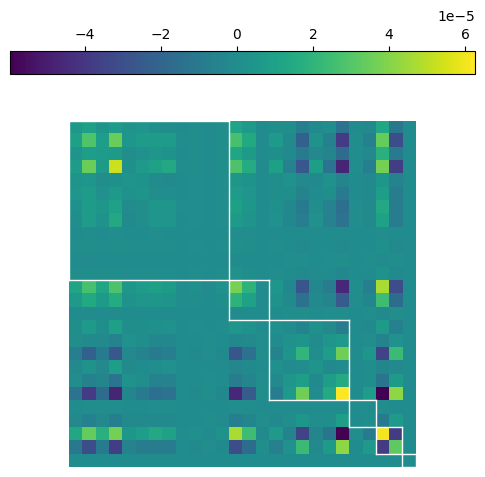
\includegraphics[width=0.43\linewidth]{../kfac_pinns_exp/exp04_gramian_contributions/fig/gram_full.png}

  \begin{minipage}[t]{0.22\linewidth}
    \centering
    Block diagonal
    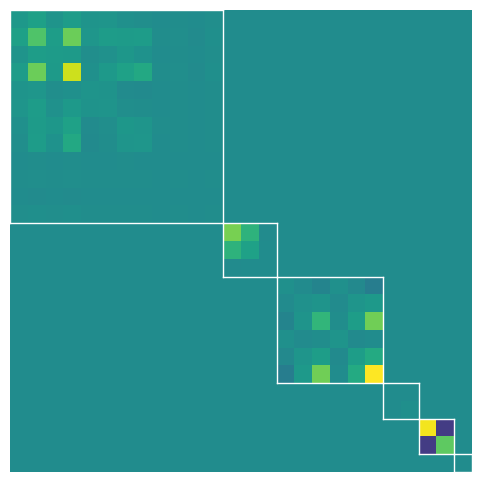
\includegraphics[width=\linewidth]{../kfac_pinns_exp/exp04_gramian_contributions/fig/gram_block_diag.png}
  \end{minipage}
  \hfill
  \begin{minipage}[t]{0.22\linewidth}
    \centering
    Summed children diagonal
    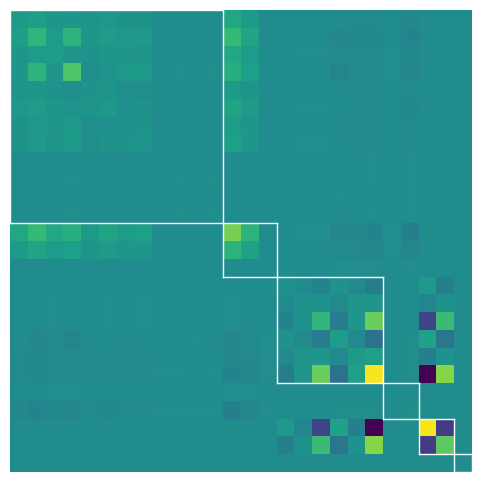
\includegraphics[width=\linewidth]{../kfac_pinns_exp/exp04_gramian_contributions/fig/gram_diag_children.png}
  \end{minipage}
  \hfill
  \begin{minipage}[t]{0.22\linewidth}
    \centering
    Summed children off-diagonal
    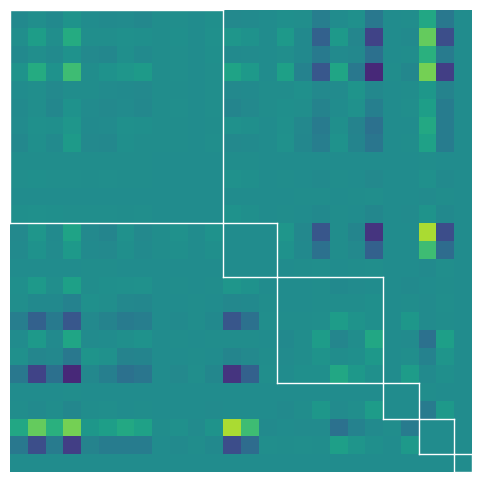
\includegraphics[width=\linewidth]{../kfac_pinns_exp/exp04_gramian_contributions/fig/gram_offdiag_children.png}
  \end{minipage}
  \caption{Contribution of terms with identical versus non-identical children to the Gramian's block diagonal.
    The strongest contribution to its block diagonal stems from the terms with identical children.}\label{fig:gramian-contribution-summed-children}
\end{figure}
%%% Local Variables:
%%% mode: latex
%%% TeX-master: "../main"
%%% End:
